% Chapter Template

\chapter{Problem Formulation} % Main chapter title

\label{Chapter3} % Change X to a consecutive number; for referencing this chapter elsewhere, use \ref{ChapterX}

\lhead{Chapter 3 \emph{Problem Formulation}} % Change X to a consecutive number; this is for the header on each page - perhaps a shortened title

\section{Motivation} \label{sec:motivation}
We consider a transformer application \cite{DBLP:journals/corr/VaswaniSPUJGKP17} which is a popular Deep Learning Neural Network pipeline for Natural Language Processing (NLP) tasks. The application exhibits ample scopes for exploiting concurrency with the possibility of executing multiple instances of standard General Matrix Multiply (GEMM) kernels in parallel. A sample DAG for one layer of the transformer network is presented in Fig. \ref{fig:motivation0}. We shall discuss necessary background and details about the workload later in the Experimental Results section.  
	\begin{figure}[ht]  
		\centering
		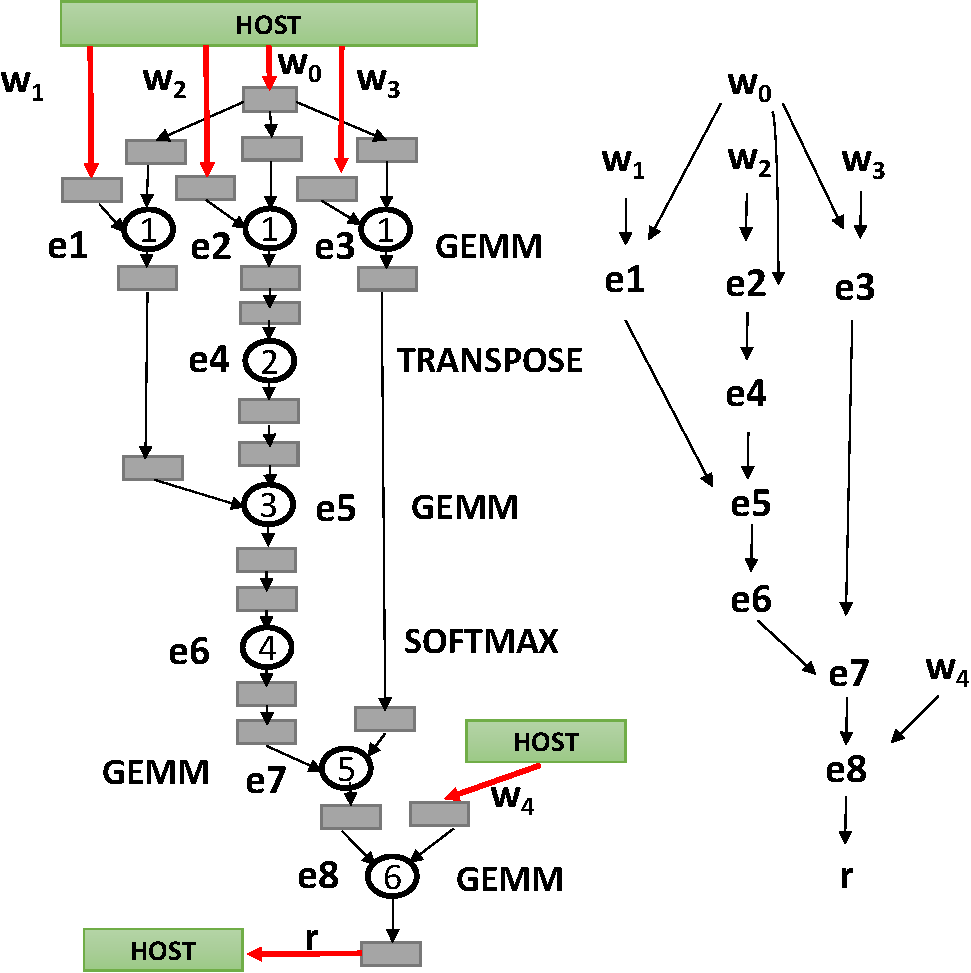
\includegraphics[scale=0.50]{Pictures/Transformer_modified.pdf}
		\caption{Event Dependencies for  DAG\label{fig:motivation0}}
	\end{figure}
	\par For the purpose of our motivation, we present a level wise view of the DAG under consideration  in the left hand side of Fig. \ref{fig:motivation0}, which contains a total of 8 kernels. As per our earlier convention, the rectangular nodes represent input output buffers and the circular nodes represent kernels Each kernel is labeled with the corresponding level number starting from 1. Initially there is a copy operation which copies the same buffer to each of the kernels at level 1.  Each of the kernels in levels 1,4,5,6 represent General Matrix Multiply (GEMM) kernels where each kernel takes as input two buffers and produces one output buffer. The kernels in level 2 and level 3 represent transpose and softmax operations respectively, each processing one input buffer to produce one output buffer. The edges between rectangular nodes i.e. buffers represent data dependencies for the DAG. For enforcing precedence constraints between any pair of  kernels $(k_i,k_j)$, a 
	programmer shall set event dependencies between read commands for output buffers of $k_i$ and write commands for input buffers of $k_j$, as was observed in Fig. \ref{fig:OpenCLArch}.  
	For our transformer DAG depicted in Fig. \ref{fig:motivation0}, the programmer is required to set event dependencies between read commands for output buffers of kernels in level $i$ and write commands for input buffers of kernels in level $i+1$. If the entire DAG was mapped to a single GPU device, explicit reads and writes for dependent buffers between kernels in levels 1-5 are not required. For this case, the programmer needs to set up event dependencies between \textit{ndrange} commands of kernels in levels $i$ and $i+1$. 
	\par In the left hand side of Fig 3. we label each kernel $k$ of the DAG with event $e_k$ associated with the corresponding \textit{ndrange} command for that kernel. Apart from this, we have a \textit{write} command $w_0$ responsible for copying one common buffer to be used for each GEMM kernel in level $1$. We also have \textit{write} commands $w_1,w_2,w_3$ for each of the remaining buffers required by GEMM kernels in level $1$ and a \textit{write} command $w_4$ for a buffer required by GEMM kernel in level $6$. Finally we have a \textit{read} command $r$ for the output buffer of the GEMM kernel in level $6$. The dependencies between these events are depicted in the corresponding event dependency graph in the right hand side of Fig. \ref{fig:motivation0}. The end designer is burdened with the task of manually writing a host program that will capture the event dependencies illustrated in this dependency graph for ensuring that precedence relations of the DAG are met during execution. This is achieved by using the complex programming constructs for OpenCL events and callback functions as discussed earlier.    
	\par We next examine how coarse-grained and fine-grained scheduling decisions are made for mapping this DAG onto a single GPU device with the help of Fig. \ref{fig:finecoarse}. 
	\begin{figure}[ht]  
		\centering
		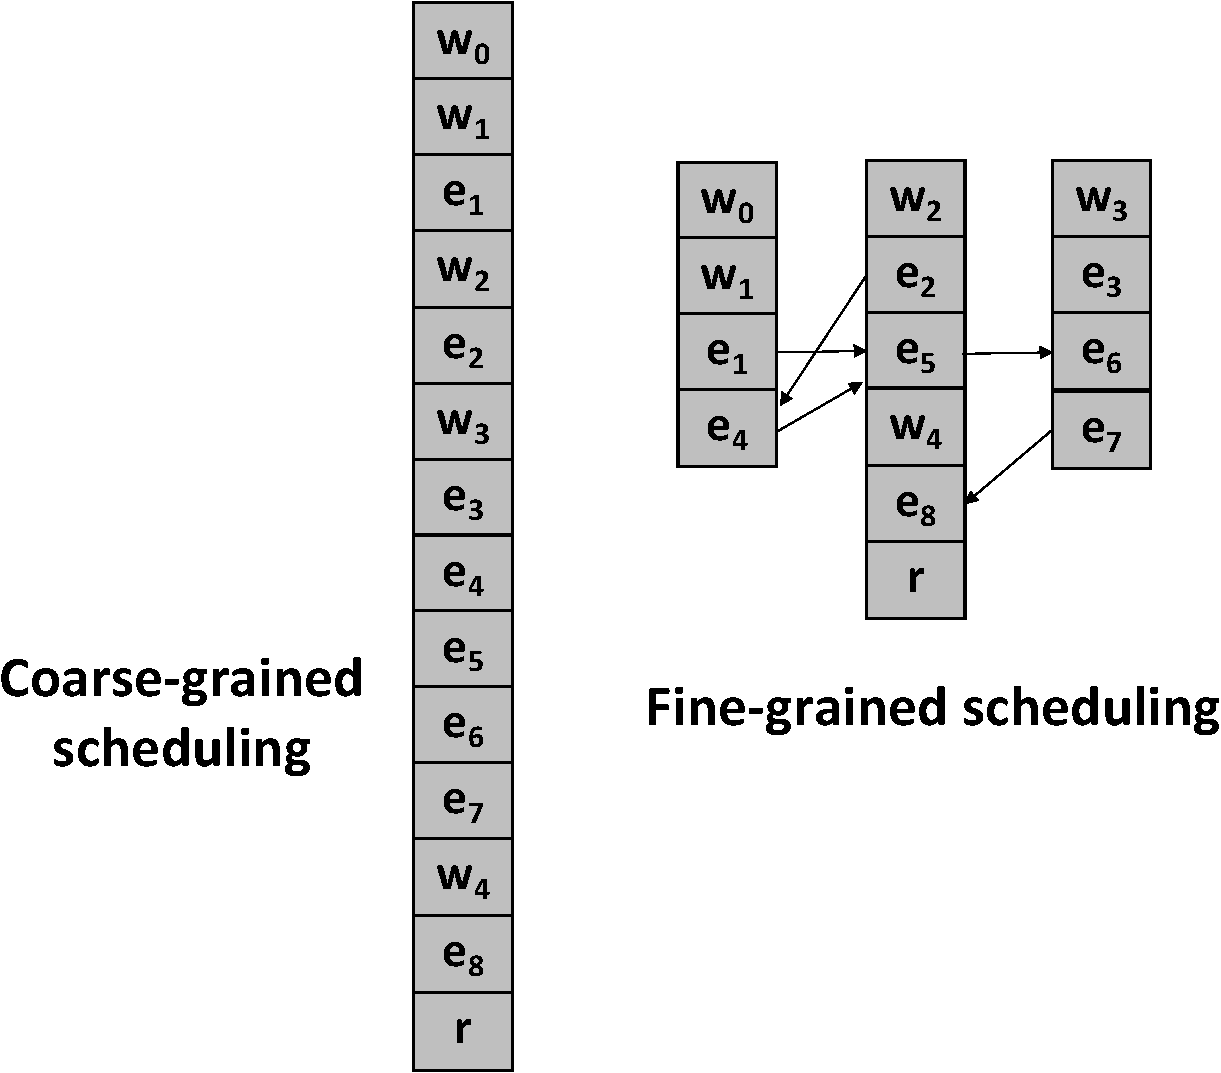
\includegraphics[scale=0.35]{Pictures/finecoarse.pdf}
		\caption{Command Queue Configurations for Scheduling \label{fig:finecoarse}}
	\end{figure}
	\par Coarse grained scheduling decisions refer to the context when all operations of kernels of a DAG are executed in its entirety first. This is achieved by setting up a single command queue on the GPU device. As a consequence, we can observe that all commands labelled by the events used in Fig. \ref{fig:motivation0} execute serially on the GPU device. In contrast if we set up multiple command queues, there is a possibility of leveraging fine grained scheduling decisions that can interleave data transfers with \textit{ndrange} operations and can execute multiple ndrange operations concurrently. In Fig. \ref{fig:finecoarse}, we setup 3 command queues for achieving this. One can observe that the writes $w_0,w_2,w_3$ can now happen simultaneously. The ndrange operations $e_1$, $e_2$ and $e_3$ can also execute concurrently on the same GPU device. However, the other commands, despite belonging to different command queues would not be able to execute simultaneously due to the precedence relationships enforced by the event dependency graph illustrated in  of Fig. \ref{fig:motivation0}.  These dependencies are represented by inter-queue edges between events in Fig. \ref{fig:finecoarse}.
	\par We note that both the cases represented in Fig. \ref{fig:finecoarse} depict one of the possible command queue configurations. In our representative example, for coarse-grained scheduling, one can have another command queue configuration where the \textit{write} command associated with $w_1$ is enqueued before that of $w_0$ or where the \textit{write} command for $w_4$ is enqueued anywhere before the \textit{ndrange} command for $e_8$. In a similar vein, one can have different command queue configurations for fine-grained scheduling as well. We next analyze how coarse-grained and fine-grained scheduling decisions for executing this DAG on a single GPU device compare with the help of the Gantt charts in Figs \ref{fig:motivation1} and \ref{fig:motivation2}. 
	\par We execute the DAG on a heterogeneous platform comprising an NVIDIA GTX-970 GPU device and a Quadcore Intel i5-4690K CPU device. The Gantt chart in Fig \ref{fig:motivation0} represents the case where a single command queue is set up for the GPU device and all the \textit{read}, \textit{write} and \textit{ndrange} commands for each of the 8 kernels are enqueued. The x-axis of the Gantt chart represents time in milliseconds (ms). The y-axis of the Gantt chart represents the kernels constituting the DAG. Each kernel is labelled with the level of the DAG to which it belongs followed by the name of the kernel operation and \textit{write}, \textit{read} and \textit{ndrange} commands pertaining to it. Each green rectangle denotes the time taken by a \textit{write} command. Each read and brown rectangle denotes the time taken by \textit{ndrange} and \textit{read} commands respectively. As evident from the corresponding Gantt chart, each command associated with each kernel executes one at a time on the GPU device resulting in an execution time of 105ms. We observe that writes occur for the first copy operation (associated with event $w0$) and for buffers of kernels in level $1$ and the kernel in level $6$. For GEMM kernels in level $1$, data is transferred for input buffers associated with events $w_1$, $w_2$ and $w_3$. Similarly for the GEMM kernel in level 6, data is transferred for the input buffer associated with event $w4$. Finally the last read associated with event $r$ occurs for the kernel in level $6$. We note that each of the operations are executed sequentially mapped to a single GPU device using a single command queue. 
	\begin{figure}[ht]  
		\centering
		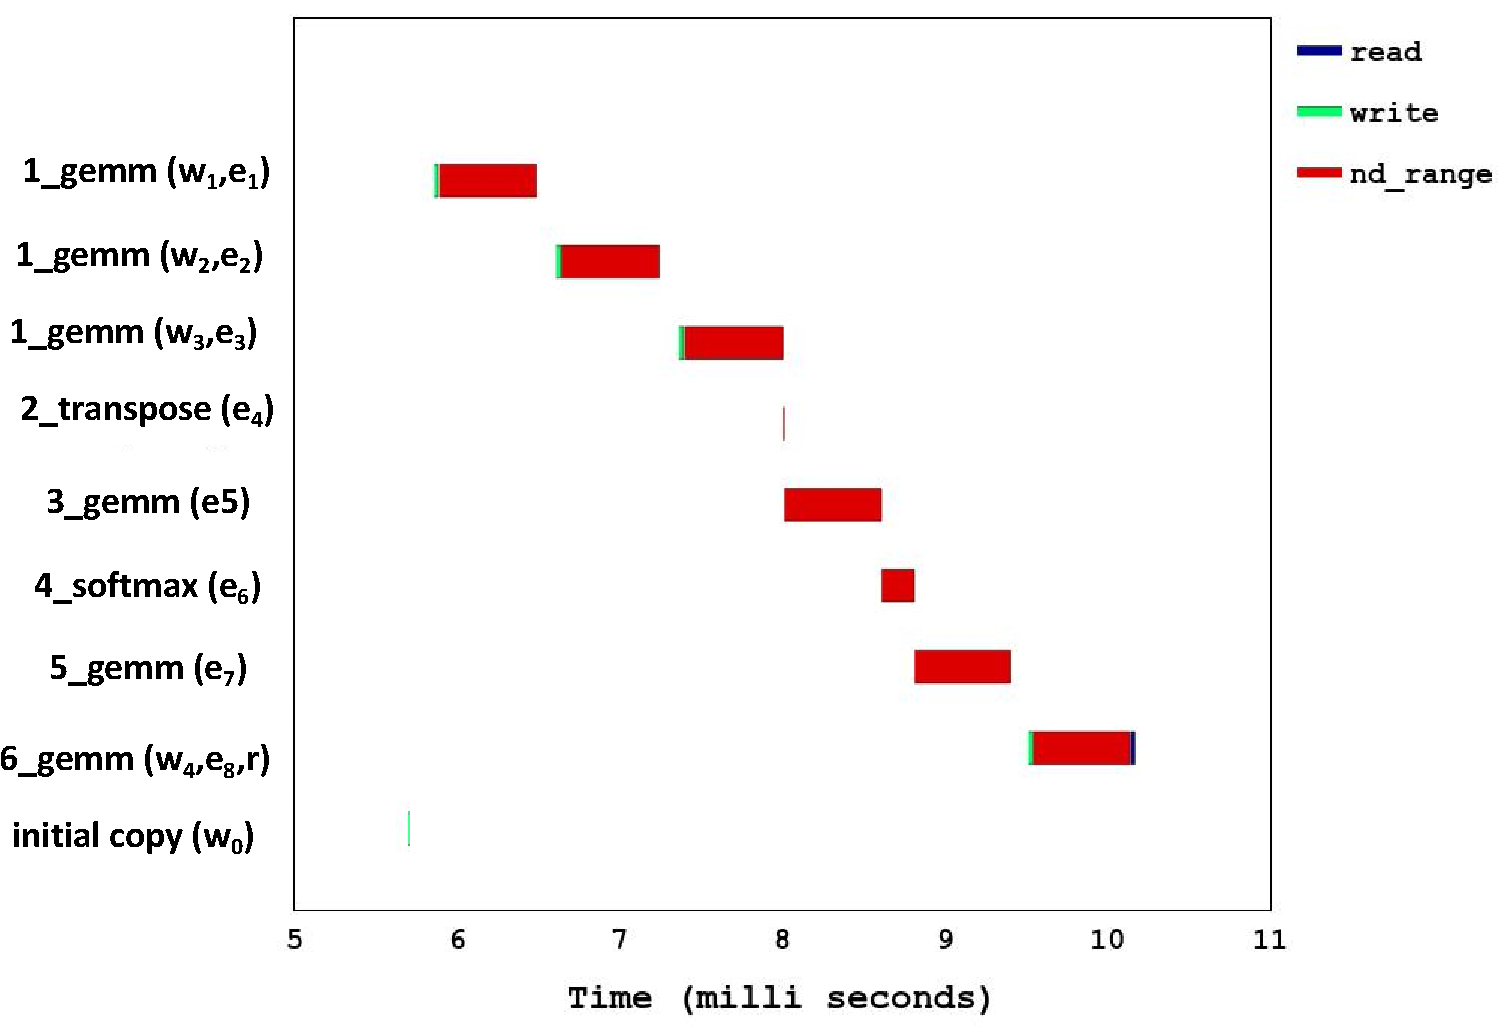
\includegraphics[scale=0.35]{Pictures/motiv_sequential.pdf}
		\caption{Sequential Execution on GPU device\label{fig:motivation1}}
	\end{figure}
	\begin{figure}[ht]  
		\centering
		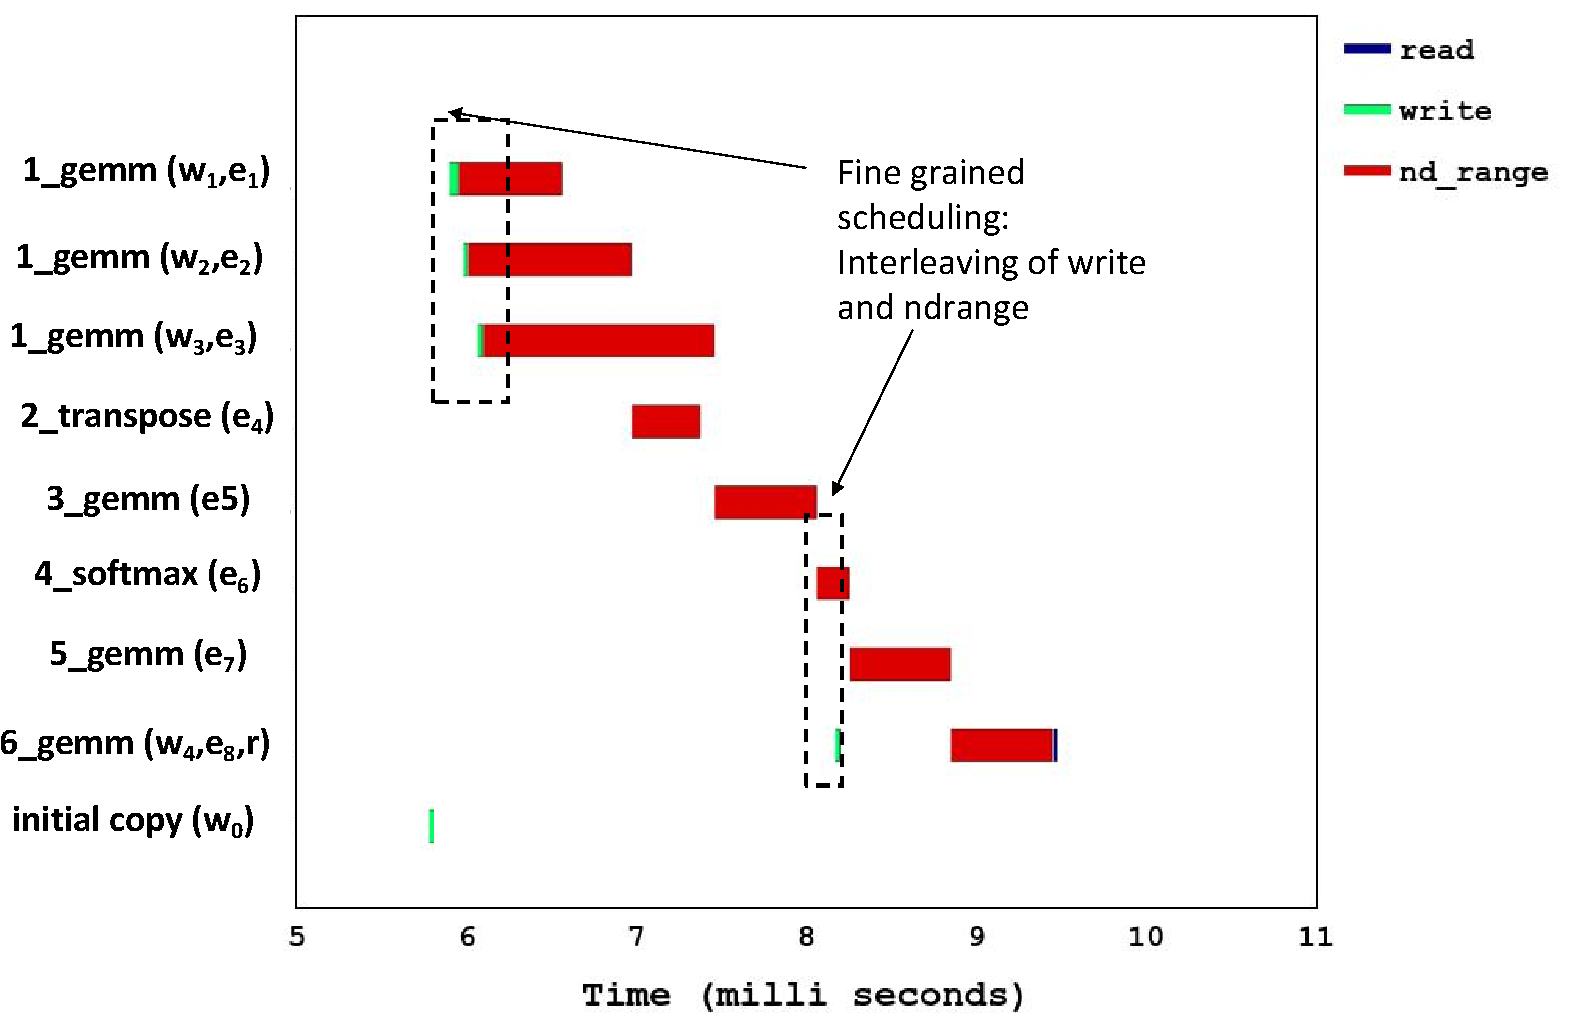
\includegraphics[scale=0.35]{Pictures/motiv_concurrent.pdf}
		\caption{Concurrent Execution on GPU device\label{fig:motivation2}}
	\end{figure}
	\par In contrast, if we set up three command queues for the same GPU device and dispatch our kernels intelligently, we observe an $8\%$ reduction in execution time , with the DAG finishing in 95ms. This reduction in time maybe attributed to the interleaving of data transfers (\textit{write} commands associated with $w1,w2$ and $w3$) with execute operations (\textit{ndrange} commands associated with events $e1,e2,e3$)  for kernels in levels $1$. It can be observed that while \textit{ndrange} command associated with $e1$ is executing, the buffer associated with $w2$ can be copied simultaneously. Similarly, $w3$ can also be copied while $e1$ and $e2$ are executing. Additionally, it can be seen that all kernels in level $1$ are  executing concurrently for the same device. It may be further observed, the individual execution times for each kernel increases slightly as a result. This is due to the fact, that different work groups of different kernels that have been concurrently dispatched  are scheduled in a round robin fashion to the compute units of the device, thus causing resource contention. However, the total time for finishing both kernels concurrently is lesser than the case when they are dispatched in sequence. We note that concurrency between three kernels and three data transfers  yields a decrease of 8 \% in execution time. In general, for one layer of the transformer a maximum of 16 such DAGs can run in parallel. In such a setting where there is more concurrency to exploit, fine grained scheduling that exploits both the CPU and the GPU devices of the heterogeneous platform by setting up multiple command queues per device shall yield more speedups.
	
	\par The typical dispatch mechanisms offered by list scheduling heuristics available in SOCL, StarPU and MultiCL are optimized for heterogeneous clusters comprising multiple devices and rely on coarse-grained scheduling decisions. They do not leverage the benefits obtained by using fine-grained scheduling decisions. We implement {\em PySchedCL} as a scheduling framework optimized for heterogeneous multicore platforms where devices support concurrent execution. Provided with the right guidance parameters by the designer, the framework shall automatically produce efficient data-parallel mapping solutions that can exploit concurrency both at the application and at the platform level.


\section{Formal Problem Statement}
\label{sec:prob}
	Let us consider a heterogeneous platform $\mathcal{P}$ depicted in Fig. \ref{fig:platprob} which comprises a CPU device and a GPU device connected via a PCI-Express bus. Each device has support for executing multiple kernels simultaneously. The OpenCL standard supports device fission for CPU devices i.e. a single CPU device can be partitioned into multiple subdevices, thereby enabling concurrent execution for the same. We consider as GPU an NVIDIA device with Hyper-Q support \cite{nvidia}. Hyper-Q offers a solution that allows the CPU host to dispatch multiple kernels simultaneously on the GPU device with the help of hardware managed work queues. 
	\par Let us represent an OpenCL application graph as a directed acyclic graph (DAG) $G = \langle K,B,E_I,E_O,E \rangle$ where $K$ denotes the set of OpenCL kernels, $B= B_I \bigcup B_O$ represents the set of buffers for all $k \in K$. The set $B_I$ denotes the set  of input buffers and the set $B_O$ denotes the set of output buffers. The set $E_I \subseteq B_I \times K$ denotes the set of edge dependencies between each input buffer and kernel, $E_O \subseteq K \times B_O$ denotes the set of edge dependencies between each kernel and output buffer. The set $E \subseteq B_O \times B_I$ denotes the set of input output buffer dependencies across kernels in the DAG. Command queues are typically setup per device depending on which kernels are mapped to which devices. 
	\begin{figure}[ht]
		\centering
		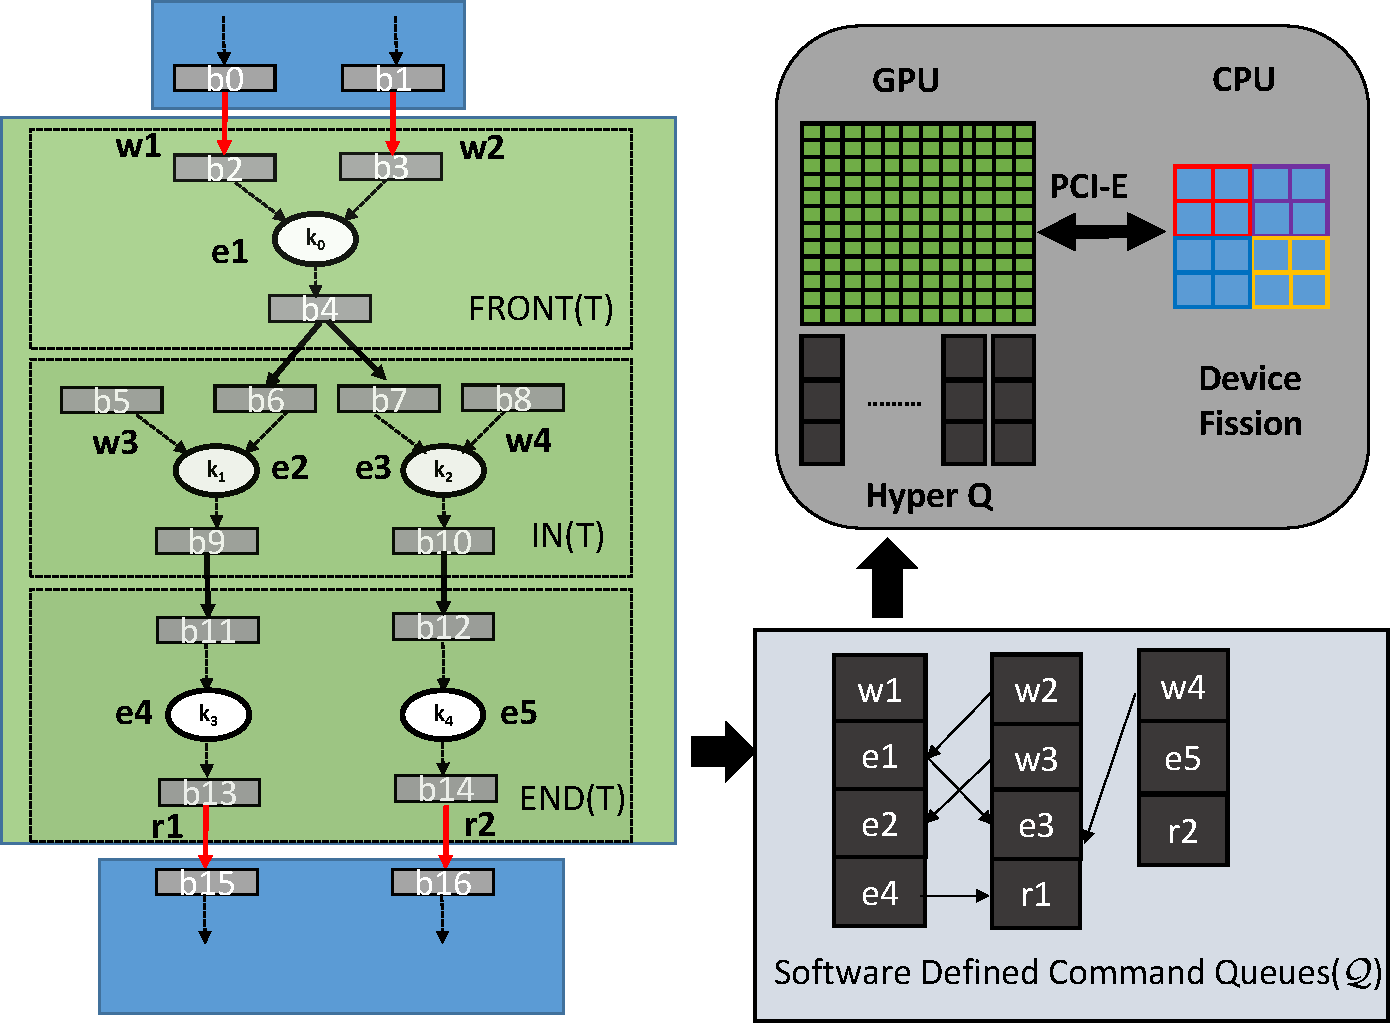
\includegraphics[scale=0.38]{Pictures/PlatformAndProblemFormulation.pdf}
		\caption{\small Platform and DAG Model\label{fig:platprob}}
	\end{figure}
	
	\begin{definition} \label{def:task-component}
		\emph{Given an OpenCL DAG $G=\langle K,B,E_I,E_O,E \rangle$, we denote a task component $T_d$ as a subset of kernels $K^\prime \subseteq K$  where each kernel $k$ is mapped to the same device $d$.} 
	\end{definition}

	\par In our case, $d= \{ cpu,gpu \}$. In Fig. \ref{fig:platprob}, we have $T_{gpu} = \{k_0,k_1,k_2,k_3,k_4 \}$. For a given task component we define the following terminology.
	\begin{definition}
		\emph{Given a task component $T_d$ pertaining to some OpenCL DAG $G$, we define $FRONT(T_d)$ as the set of kernels where each kernel $k$ has input buffer dependencies $(b_i,k) \in E_I$ such that for $b_i$, if there exists an immediate predecessor $b_j$ where $(b_j,b_i)\in E$ and $(k^\prime,b_j) \in E_O$, then the kernel $k^\prime$ belongs to a different task component $T^\prime_{d'}$.} 
	\end{definition}
	In Fig. \ref{fig:platprob}, we observe that $FRONT(T) = \{ k_0\}$, since both input buffers $b2$ and $b3$ have predecessors pertaining to kernels belonging in a different task component. 
	\begin{definition}\emph{
		Given a task component $T$ pertaining to some OpenCL DAG $G$, we define $END(T)$ as the set of kernels where each kernel $k$ has output buffer dependencies ($k,b_i) \in E_O$ such that for $b_i$ if there exists an immediate successor $b_j$ where $(b_i,b_j)\in E$ and $(b_j,k^\prime) \in E_I$ then kernel $k^\prime$ belongs to a different task component $T^\prime_{d'}$.}
	\end{definition}
	In Fig. \ref{fig:platprob}, we can observe that $END(T_{gpu})=\{k_3,k_4\}$, since both output buffers $b13$ and $b14$ are used as inputs for kernels belonging to a different task component.
	\begin{definition}\emph{
		Given a task component $T_d$ pertaining to some OpenCL DAG $G$, we define $IN(T)$ as the set of kernels where each kernel $k \in T_d, k \notin FRONT(T), k \notin END(T)$. } 
	\end{definition}
	In Fig. \ref{fig:platprob}, we can observe that $IN(T)=\{k_1, k_2 \}$
	
	We classify buffer edge dependencies $(b_i,b_j) \in E$ into two categories -i) intra-edge, ii) inter-edge.
	\begin{definition}\emph{
		Given a task component $T_d$ pertaining to a DAG $G$, an edge $(b_i,b_j)$ is said to be intra-edge if there exists kernels $k_i,k_j$ such that $(k_i,b_i) \in E_O$, $(b_j,k_j) \in E_I$ and both kernels $k_i,k_j$ belong to the same component.} 
	\end{definition}
	In Fig. \ref{fig:platprob}, we can observe that $(b4,b6)$ and $(b4,b7)$ are intra-edges for $T_{gpu}$.
	\begin{definition}\emph{
		Given two task components $T_x$ and $T_y$ pertaining to a DAG $G$, an edge $(b_i,b_j)$ is said to be an inter-edge from $T_x$ to $T_y$ if there exists kernels $k_i,k_j$ such that $(k_i,b_i) \in E_O$, $(b_j,k_j) \in E_I$ and kernel $k_i$ belongs to $T_x$ and $k_j$ belongs to $T_y$.}
	\end{definition}
	In Fig. \ref{fig:platprob}, we can observe that $(b0,b2)$, $(b1,b3)$, $(b13,b15)$ and $(b15,b16)$ are inter-edges.
	We classify kernel-buffer dependencies in $E_I$ and $E_O$ into two categories - i) isolated copy and ii) dependent copy
	\begin{definition}\emph{
		Given any kernel $k_i$, an edge ($b_i,k_i)\in E_I$ represents an isolated copy (write) {\em iff} for every $b_k \in B$, $(b_k,b_i) \notin E$.
		In a similar fashion, an edge ($k_i,b_j)$ represents an isolated copy(read) {\em iff} for every $b_k \in B$, $(b_j,b_k) \notin E$ respectively.}
	\end{definition}
	In Fig. \ref{fig:platprob}, the edges $(b5,k_1)$ and $(b8,k_2)$ correspond to isolated writes. 
	\begin{definition}\emph{
		Given any kernel $k_i$ pertaining to a task component $T_d$, an edge ($b_i,k_i)\in E_I$ represents a dependent copy (write) {\em iff} there exists some buffer $b_i \in B$ such that  $(b_i,b_k)\in E$.
		In a similar fashion, an edge ($k_i,b_i$) represents a dependent copy(read) {\em iff} there exists some $b_k \in B$ such that $(b_j,b_k) \in E$.} 
	\end{definition}
	In Fig. \ref{fig:platprob}, every buffer-kernel dependency apart from $(b5,k_1)$ and $(b8,k_2)$ correspond to dependent copies.
	\begin{definition}\emph{
		Given a task component $T_d$ of an application DAG $G$ mapped to a device $d$ with $r$ command queues, we define the command queue data structure $\mathcal{Q}$ as a graph $\langle V_Q, E_Q\rangle$  where $V_Q=\{q_1,q_2,\cdots,q_r\}$ denotes the set of command queues allocated to $T_d$. Each element $o_i$ belonging to each queue $q_i$ constitutes either a \textit{write}, \textit{ndrange} or \textit{read} operation pertaining to some kernel belonging to $T_d$. Each element of the set $E_Q$ is an edge of the form $\langle o_i,o_j \rangle$ where  $o_i \in q_r$ and $o_j \in q_s$ such that  $q_r \neq q_s$ and represents the precedence constraints enforced by the edges in the DAG $G$. }
	\end{definition}
	The framework uses an $enq$ procedure that sets up the data structure $\mathcal{Q}$ for task component $T_d$ as follows.
	An operation $o_i$ pertaining to kernel $k_i$  is enqueued to one of the command queues in $V_Q$ depending upon the membership of $k_i$ in the sets $IN(T_d)$, $FRONT(T_d)$ and $END(T_d)$. This is described below.
	\par \noindent i)If $k_i \in FRONT(T_d)$, the enqueue procedure $enq$ enqueues all dependent write commands for buffers $b_j$ corresponding to dependent writes $(b_j,k_i) \in E_I$ followed by the ndrange command for $k_i$.
	\par \noindent ii) If $k_i \in END(T_d)$, the enqueue procedure $enq$ enqueues the ndrange command for $k_i$ followed by all dependent read commands for buffers $b_j$ corresponding to intra-edges $k_i,b_j \in E_O$.  
	\par \noindent iii) If $k_i \in IN(T_d)$, the enqueue procedure $enq$ enqueues only the ndrange command for $k_i$ 
	\par \noindent iv) For every kernel $k_i$  belonging to $FRONT(T)$, $IN(T) $and $END(T)$, the enqueue procedure $enq$ enqueues all isolated writes for input buffers $b_j$, $(b_j,k_i) \in E_I$ before enqueuing the ndrange command for $k_i$ and all isolated reads for output buffers $b_r$, $(k_i,b_r) \in E_O$ after enqueueing the ndrange command for $k_i$. 
	\par An edge $(o_i,o_j) \in E_Q$ exists if i) $o_i$ is a isolated/dependent write $(b_r,k_s)$ and $o_j$ is an ndrange operation for kernel $k_s$ ii) $o_i$ is an ndrange operation for kernel $k_s$ and $o_s$ is a dependent/isolated write $(k_s,b_r)$ and iii)both $o_i$ and $o_j$ are ndrange operations for kernels $k_r$ and $k_s$ respectively such that there exists edges $(k_r,b_r) \in E_O$, $(b_s,k_s) \in E_I$  and $(b_r,b_s) \in E$ is an intra edge. In Fig. \ref{fig:platprob}, $(b_3,k_0)$ corresponds to a dependent write for kernel $k_0$ thus requiring a dependency between associated operations $w_2$ and $e_1$ in $\mathcal{Q}$.  The edge $(e_1,e_3)$ represents the dependency between kernels $k_0$ and $k_2$ arising due to the dependencies $(k_0,b_4)$,$(b4_b7)$,$(b_7,k_2)$ where $b_4,b_7$ is an inter edge. 
	\par The framework expects that the device preferences for each kernel are known beforehand. Using this information and the $enq$ procedure, the framework can emulate dynamic coarse-grained scheduling decisions supported by frameworks like StarPU and SOCL where kernels are dispatched one at a time to devices. For fine-grained scheduling algorithms it is expected that the user provides an initial decomposition of the DAG $G$ into a set of task components $\mathcal{T}$ where each task component $T_d \in \mathcal{T} \in \mathcal{T} $ is mapped to a particular device $d$. Additionally, one must provide as guidance parameters for each task component $T_d$, the number of command queues to be used. Given this as input, the framework automatically sets up multiple command queues inside each task component for  device $d$ and outputs a schedule $\sigma$ which is an ordered sequence of $enq$ procedures that respects the precedence relationships of the application DAG. The problem formulation is formally stated as follows.
	\begin{definition}\emph{
		Given a DAG $G = \langle K,B,E_I,E_O,E \rangle$,  a corresponding set of $m$ task components $\mathcal{T} = \lbrace T_{d_1}, T_{d_2}, \cdots, T_{d_p}\rbrace$ and a target heterogeneous CPU-GPU multicore platform $\mathcal{P} = \{d_1,d_2,\cdots d_p \}$ containing $p$ devices, a schedule $\sigma$ is an ordered sequence of enqueue procedures $enq(T_{d_1}), enq(T_{d_2}),\cdots,enq(T_{d_p})$ such that the kernels $k_i \in K$ is dispatched in a topologically sorted fashion i.e sorted with respect to the ordering of $k_i$'s enforced by the edges in $G$,  $k_1 \preceq k_2 \preceq \cdots, k_{|K|}$. } 
	\end{definition}
	